\documentclass[10pt,a4paper,titlepage]{article}
\usepackage[utf8]{inputenc}
\usepackage{amsmath}
\usepackage{amsfonts}
\usepackage{amssymb}
\usepackage[ngerman]{babel}
\usepackage[pdftex]{graphicx}
\usepackage[vmargin=3cm, hmargin=2cm]{geometry}
\usepackage{tabularx}
\usepackage{color}
\usepackage{fancyvrb}
\usepackage{pdflscape}

\setlength{\parindent}{0pt}
\setlength{\parskip}{2pt}

\title{Validierung}
\author{Simon Bischof \and Jan Haag \and Adrian Herrmann \and Lin Jin \and Tobias Schlumberger \and Matthias Schnetz}

\makeindex

\begin{document}

\thispagestyle{empty}
\vspace*{4cm}
\begin{center}
\begin {huge}
Validierung\\
\end{huge}
Simon Bischof, Jan Haag, Adrian Herrmann, Lin Jin, Tobias Schlumberger, Matthias Schnetz\\
\vspace{3cm}
\begin{huge}
Praxis der Softwareentwicklung \\
Projekt 3:\\
Automatisches Pr\"{u}fen der Korrektheit von Programmen\\
Gruppe 1\\
\vspace{2cm}

\includegraphics[height=2cm]{images/Logo.pdf}\\[0.5cm]
\end{huge}
\begin{huge}
WS 2011/2012
\end{huge}
\end{center}
\newpage
\tableofcontents
\newpage

\section{Gesamt"uberdeckung}
Eine "Ubersicht der erreichten Anweisungs- und Zweig"uberdeckung aus den Unit-, System- und Integrationstests. Details sind im "Uberdeckungsbericht zu finden. \\[0.5cm]
\begin{tabular}{|p{3cm}|p{1.5cm}|p{2.5cm}|p{1.5cm}|p{1.5cm}|p{2.5cm}|p{1.5cm}|}
\hline
& \multicolumn{3}{c|}{Anweisung} & \multicolumn{3}{c|}{Zweig} \\ 
\hline
Paket&Cov.&Gesamt-&nicht&Cov.&Gesamt-&nicht\\
&&anzahl&"uberdeckt&&anzahl&"uberdeckt \\\hline
AST&100\%&1639&0&100\%&154&0 \\\hline
Parser&92\%&13733&1069&69\%&1432&439 \\\hline
Interpreter&100\%&2445&12&98\%&272&6 \\\hline
Verifier&85\%&328&48&94\%&16&1 \\\hline
SMTLib&99\%&2744&27&96\%&138&5 \\\hline
Z3&56\%&5026&2217&42\%&632&367 \\\hline
GUI&97\%&4193&138&79\%&112&23 \\\hline
GUI-Controller&98\%&3378&60&87\%&336&43 \\\hline
Misc&92\%&2549&200&89\%&206&22 \\\hline
Insgesamt&91\%&47521&4498&72\%&3228&908 \\\hline
\end{tabular}

\section{Ergebnisse der Tests}
Als Bugtracker haben wir Git benutzt, indem f"ur jeden Bug ein neuer Issue ge"offnet wird. Insgesamt wurden 112 Bugs gefunden. Davon sind 107 bereits behoben und 5 offen, die aus zeitlichen Gr"unden nicht mehr bearbeitet werden konnten. \\[0.5cm]
Die Verteilung sieht wie folgt aus: \\[0.2cm]
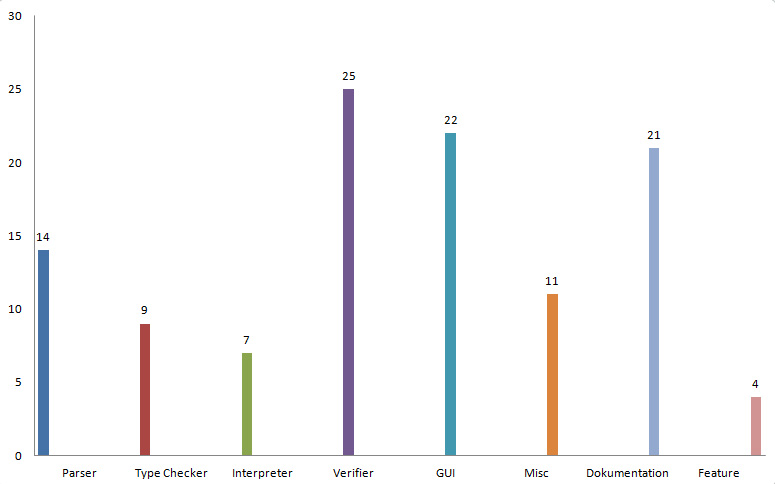
\includegraphics[width=18cm]{images/closed} \\
Und die Verteilung der noch offenen Issues: \\
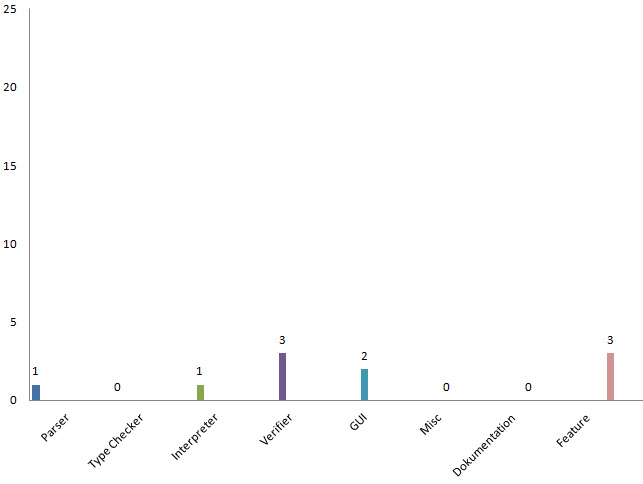
\includegraphics[width=15cm]{images/open}

\section{Testszenarien aus dem Pflichtenheft}
Alle Testf"alle aus dem Pflichtenheft konnten erfolgreich durchgef"uhrt werden. Dabei gab es allerdings zwei kleine "Anderungen: 
\begin{itemize}
\item Das Schl"usselwort \texttt{require} wurde in \texttt{assume} umbenannt.
\item Wir haben uns gegen Laufzeitfehler entschieden und stattdessen Assertions bei Division durch 0 und Arrayzugriffen eingef"ugt, weswegen die erwarteten Laufzeitfehler aus dem Pflichtenheft durch Assertionfailures ersetzt wurden .
\end{itemize}

\section{Kompatibilit"atstests}
Wir haben das Programm auf den folgenden Betriebssystemen getestet und haben keine Kompatibilit"atsprobleme entdeckt:
\begin{itemize}
\item Windows 7
\item Windows XP
\item Linux
\item Mac OS
\end{itemize}

\section{Performancetests}
Die folgenden Tests haben wir durchgef"uhrt:
\begin{itemize}
\item Langes flaches Program mit Zuweisungen
\begin{itemize}
\item Laden: 10,02s
\item Ausf"uhren: 0,336s
\end{itemize}
\item Langes verschachteltes Program
\begin{itemize}
\item Laden: 9,45s
\item Ausf"uhren: 0,4s
\end{itemize}
\item Langes Program mit komplizierten Berechnungen
\begin{itemize}
\item Laden: 458,2s
\item Ausf"uhren: 3,45s
\end{itemize}
\item Z"ahlschleife \\[0.2cm]
\begin{tabular}{|p{3cm}|p{3cm}|p{3cm}|}
\hline
Anzahl Durchl"aufe&Ben"otigte Zeit&Java Vergleich \\\hline
100&$<$500ms&1.500ns\\\hline
1.000&$<$1s&6.000ns\\\hline
10.000&$<$1s&12.000ns\\\hline
100.000&$<$1s&90.000ns\\\hline
1.000.000&4s&0,8ms\\\hline
10.000.000&35s&8ms\\\hline
100.000.000&6min&76ms\\\hline
\end{tabular}
\\[0.2cm]
Ungef"ahr um Faktor 5 langsamer als JVM
\item Russische Multiplikation
\begin{itemize}
\item Verifizieren: 0,15s
\end{itemize}
\item Einfaches Program mit Funktionsaufruf
\begin{itemize}
\item Verifizieren: 0,08s
\end{itemize}
\item Kleines Program mit Ergebnis "`unknown"'
\begin{itemize}
\item Verifizieren: 24,58s
\end{itemize}
\end{itemize}

\section{GUI Testplan}
\subsection{Menubar}
\subsubsection{"`File"' $\rightarrow$ "`New"'}
\begin{enumerate}
\item "Offnen einer neuen Datei
\begin{itemize}
\item Erwartetes Ereignis: Der Inhalt des Editors wird ohne zu speichern gel"oscht, Breakpoints werden entfernt und die Konsolen geleert. 
\item Status: \textcolor{red}{FEHLSCHLAG} \\
Breakpoints werden nicht entfernt, Konsole nicht geleert
\end{itemize}
\end{enumerate}
\subsubsection{"`File"' $\rightarrow$ "`Load"'}
\begin{enumerate}
\item Laden einer nichtexistenten Datei
\begin{itemize}
\item Erwartetes Ereignis: Die Datei wird nicht geladen. 
\item Status: \textcolor{green}{OK} 
\end{itemize}
\item Laden einer Datei, die vom Programm erzeugt wurde
\begin{itemize}
\item Erwartetes Ereignis: Die ausgew"ahlte Datei wird in den Editor geladen. 
\item Status: \textcolor{green}{OK}
\end{itemize}
\item Laden einer reinen Textdatei (zum Beispiel: txt, tex)
\begin{itemize}
\item Erwartetes Ereignis: Die ausgew"ahlte Datei wird in den Editor geladen. 
\item Status: \textcolor{green}{OK}
\end{itemize}
\item Laden einer durch Textbearbeitungsprogramme erstellten Textdatei (Getestet: docx, pdf)
\begin{itemize}
\item Erwartetes Ereignis: Die Datei wird nicht geladen. 
\item Status: \textcolor{red}{FEHLSCHLAG} \\
docx-Dateien werden geladen, Programm h"angt sich auf bei pdf-Dateien
\end{itemize}
\item Laden einer Nichttextdatei (zum Beispiel: exe)
\begin{itemize}
\item Erwartetes Ereignis: Die Datei wird nicht geladen. 
\item Status: \textcolor{red}{FEHLSCHLAG} \\
Programm h"angt sich auf
\end{itemize}
\item Nachdem eine Datei korrekt geladen wurde
\begin{itemize}
\item Erwartetes Ereignis: Der alte Inhalt des Editors wird ohne zu speichern gel"oscht, Breakpoints werden entfernt und die Konsolen geleert. 
\item Status: \textcolor{red}{FEHLSCHLAG} \\
Breakpoints werden nicht entfernt, Konsole nicht geleert
\end{itemize}
\end{enumerate}
\subsubsection{"`File"' $\rightarrow$ "`Save"'}
\begin{enumerate}
\item Speichern in einer nichtexistenten Datei
\begin{itemize}
\item Erwartetes Ereignis: Die Datei wird erzeugt, der Inhalt des Editors darin gespreichert. 
\item Status: \textcolor{green}{OK} 
\end{itemize}
\item Speichern in einer vom Programm erzeugten Datei
\begin{itemize}
\item Erwartetes Ereignis: Der Inhalt der Datei wird durch den des Editors ersetzt. 
\item Status: \textcolor{green}{OK} 
\end{itemize}
\item Speichern in einer reinen Textdatei
\begin{itemize}
\item Erwartetes Ereignis: Der Inhalt der Datei wird durch den des Editors ersetzt. 
\item Status: \textcolor{green}{OK} 
\end{itemize}
\item Speichern in einer durch Textbearbeitungsprogramme erstellten Textdatei (zum Beispiel: docx, pdf)
\begin{itemize}
\item Erwartetes Ereignis: Die Datei wird nicht gespeichert. 
\item Status: \textcolor{red}{FEHLSCHLAG} \\
Die Datei wird gespeichert.
\end{itemize}
\item Speichern in einer Nichttextdatei (zum Beispiel: exe)
\begin{itemize}
\item Erwartetes Ereignis: Die Datei wird nicht gespeichert. 
\item Status: \textcolor{red}{FEHLSCHLAG} \\
Die Datei wird gespeichert.
\end{itemize}
\end{enumerate}
\subsubsection{"`File"' $\rightarrow$ "`Exit"'}
\begin{enumerate}
\item Beenden des Programms
\begin{itemize}
\item Erwartetes Ereignis: Das Programm wird sofort beendet. 
\item Status: \textcolor{green}{OK}
\end{itemize}
\end{enumerate}
\subsubsection{"`Edit"' $\rightarrow$ "`Undo"'}
\begin{enumerate}
\item R"uckg"angigmachen des zuletzt eingetippten Zeichen
\begin{itemize}
\item Erwartetes Ereignis: Das zuletzt eingetippte Zeichen wird gel"oscht. 
\item Status: \textcolor{green}{OK}
\end{itemize}
\item Beliebige Wiederholung von Punkt 1
\begin{itemize}
\item Erwartetes Ereignis: Die zuletzt eingetippten Zeichen werden gel"oscht. 
\item Status: \textcolor{green}{OK}
\end{itemize}
\item R"uckg"angigmachen des zuletzt gel"oschten Zeichen
\begin{itemize}
\item Erwartetes Ereignis: Das zuletzt gel"oschte Zeichen wird wieder hergestellt. 
\item Status: \textcolor{red}{FEHLSCHLAG} \\
Punkt 4 funktioniert bis auf das zuerst gel"oschte Zeichen
\end{itemize}
\item Beliebige Wiederholung von Punkt 3
\begin{itemize}
\item Erwartetes Ereignis: Die zuletzt gel"oschten Zeichen werden wieder hergestellt. 
\item Status: \textcolor{green}{OK}
\end{itemize}
\item R"uckg"angigmachen der letzten Paste-Aktion
\begin{itemize}
\item Erwartetes Ereignis: Die zuletzt eingef"ugte Zeichenkette wird gel"oscht. 
\item Status: \textcolor{green}{OK}
\end{itemize}
\item Beliebige Wiederholung von Punkt 5
\begin{itemize}
\item Erwartetes Ereignis: Die zuletzt eingef"ugten Zeichenketten werden gel"oscht. 
\item Status: \textcolor{green}{OK}
\end{itemize}
\item R"uckg"angigmachen der letzten Cut-Aktion
\begin{itemize}
\item Erwartetes Ereignis: Die zuletzt gel"oschte Zeichenkette wird wieder hergestellt. 
\item Status: \textcolor{green}{OK}
\end{itemize}
\item Beliebige Wiederholung von Punkt 7
\begin{itemize}
\item Erwartetes Ereignis: Die zuletzt gel"oschten Zeichenketten werden wieder hergestellt. 
\item Status: \textcolor{green}{OK}
\end{itemize}
\item R"uckg"angigmachen der Funktion "`File"' $\rightarrow$ "`New"'
\begin{itemize}
\item Erwartetes Ereignis: Der alte Inhalt des Editors wird wieder hergestellt. 
\item Status: \textcolor{green}{OK}
\end{itemize}
\item Punkt 9 nachdem mehrmals auf "`File"' $\rightarrow$ "`New"' geklickt wurde
\begin{itemize}
\item Erwartetes Ereignis: Der alte Inhalt des Editors wird wieder hergestellt. 
\item Status: \textcolor{red}{FEHLSCHLAG} \\
Das erwartete Ereignis passiert erst nach dem zweiten Undo
\end{itemize}
\item R"uckg"angigmachen der Funktion "`File"' $\rightarrow$ "`Load"'
\begin{itemize}
\item Erwartetes Ereignis: Der alte Inhalt des Editors wird wieder hergestellt. 
\item Status: \textcolor{green}{OK}
\end{itemize}
\item Punkt 11 nachdem mehrmals "`File"' $\rightarrow$ "`Load"' benutzt wurde
\begin{itemize}
\item Erwartetes Ereignis: Der Inhalt der zuletzt geladenen Datei wird im Editor hergestellt. 
\item Status: \textcolor{red}{FEHLSCHLAG} \\
Der Inhalt vor den Load-Vorg"angen wird nach dem zweiten Undo hergestellt
\end{itemize}
\item Undo, obwohl noch keine Aktion aufgef"uhrt wurde
\begin{itemize}
\item Erwartetes Ereignis: Es passiert nichts. 
\item Status: \textcolor{green}{OK}
\end{itemize}
\end{enumerate}
\subsubsection{"`Edit"' $\rightarrow$ "`Redo"'}
\begin{enumerate}
\item R"uckg"angigmachen der letzten Undo-Aktion
\begin{itemize}
\item Erwartetes Ereignis: Die r"uckg"angig gemachte Aktion wird hergestellt. 
\item Status: \textcolor{green}{OK}
\end{itemize}
\item Beliebige Wiederholung von Punkt 1
\begin{itemize}
\item Erwartetes Ereignis: Die r"uckg"angig gemachten Aktionen werden hergestellt. 
\item Status: \textcolor{green}{OK}
\end{itemize}
\end{enumerate}
\subsubsection{"`Edit"' $\rightarrow$ "`Cut"'}
\begin{enumerate}
\item L"oschen der markierten Zeichenkette
\begin{itemize}
\item Erwartetes Ereignis: Die markierte Zeichenkette wird gel"oscht. 
\item Status: \textcolor{green}{OK}
\end{itemize}
\item Cut ohne markierte Zeichenkette
\begin{itemize}
\item Erwartetes Ereignis: Es passiert nichts. 
\item Status: \textcolor{red}{FEHLSCHLAG} \\
Programm st"urzt ab.
\end{itemize}
\end{enumerate}
\subsubsection{"`Edit"' $\rightarrow$ "`Copy"'}
\begin{enumerate}
\item Kopieren der markierten Zeichenkette
\begin{itemize}
\item Erwartetes Ereignis: Die markierte Zeichenkette wird zum Kopieren gespeichert. 
\item Status: \textcolor{green}{OK}
\end{itemize}
\item Beliebige Wiederholung von Punkt 1
\begin{itemize}
\item Erwartetes Ereignis: Die zuletzt kopierte Zeichenkette wird gespeichert. 
\item Status: \textcolor{green}{OK}
\end{itemize}
\item Copy ohne markierte Zeichenkette
\begin{itemize}
\item Erwartetes Ereignis: Es passiert nichts. 
\item Status: \textcolor{red}{FEHLSCHLAG} \\
Programm st"urzt ab.
\end{itemize}
\end{enumerate}
\subsubsection{"`Edit"' $\rightarrow$ "`Paste"'}
\begin{enumerate}
\item Einf"ugen der aus dem Programm kopierten Zeichenkette
\begin{itemize}
\item Erwartetes Ereignis: Die kopierte Zeichenkette wird im Editor eingef"ugt. 
\item Status: \textcolor{green}{OK}
\end{itemize}
\item Einf"ugen der aus einem anderen Programm kopierten Zeichenkette
\begin{itemize}
\item Erwartetes Ereignis: Die kopierte Zeichenkette wird im Editor eingef"ugt. 
\item Status: \textcolor{green}{OK}
\end{itemize}
\item Beliebige Wiederholung von Punkt 1 oder 2
\begin{itemize}
\item Erwartetes Ereignis: Die kopierte Zeichenkette wird jedes Mal im Editor eingef"ugt. 
\item Status: \textcolor{green}{OK}
\end{itemize}
\end{enumerate}
\subsubsection{"`Edit"' $\rightarrow$ "`Settings"'}
\begin{enumerate}
\item "Offnen des Settingsfensters
\begin{itemize}
\item Erwartetes Ereignis: Das Fenster zur Einstellung von Z3-Settings wird ge"offnet. 
\item Status: \textcolor{green}{OK}
\end{itemize}
\end{enumerate}
\subsubsection{"`Run"' $\rightarrow$ "`Run"'}
Siehe Abschnitt 1.4.2
\subsubsection{"`Run"' $\rightarrow$ "`Single Step"'}
Siehe Abschnitt 1.4.3
\subsubsection{"`Run"' $\rightarrow$ "`Random Test"'}
\begin{enumerate}
\item "Offnen des Randomtestfensters
\begin{itemize}
\item Erwartetes Ereignis: Das Fenster f"ur Randomtests wird ge"offnet. 
\item Status: \textcolor{green}{OK}
\end{itemize}
\end{enumerate}
\subsubsection{"`Run"' $\rightarrow$ "`Verify"'}
Siehe Abschnitt 1.4.6
\subsubsection{"`Help"' $\rightarrow$ "`Help"'}
\begin{enumerate}
\item "Offnen des Helpfensters und Anzeigen der Helpdokumentation
\begin{itemize}
\item Erwartetes Ereignis: Die Helpdokumentation wird ge"offnet. 
\item Status: \textcolor{green}{OK}
\end{itemize}
\end{enumerate}
\subsubsection{"`Help"' $\rightarrow$ "`About"'}
\begin{enumerate}
\item "Offnen des Aboutfensters
\begin{itemize}
\item Erwartetes Ereignis: Das Aboutfenster wird ge"offnet. 
\item Status: \textcolor{green}{OK}
\end{itemize}
\end{enumerate}

\subsection{Frames}
\subsubsection{Settingsframe}
\begin{enumerate}
\item Speichern von korrekten Eingaben
\begin{itemize}
\item Erwartetes Ereignis: Es wird eine Erfolgsmeldung ausgegeben und die neuen Eingaben stehen in den entsprechenden Textfeldern.
\item Status: \textcolor{green}{OK}
\end{itemize}
\item Speichern von inkorrekten Eingaben
\begin{itemize}
\item Erwartetes Ereignis: Es wird eine Fehlermeldung ausgegeben und die alten Werte werden wiederhergestellt.  
\item Status: \textcolor{blue}{BEHOBEN} \\
Wenn der Pfad nicht korrekt eingegeben wurde, wird trotzdem die Erfolgsmeldung angezeigt.
\end{itemize}
\item Klick auf "`Close"' Button
\begin{itemize}
\item Erwartetes Ereignis: Das Settingsframe wird geschlossen.
\item Status: \textcolor{green}{OK}
\end{itemize}
\item Ausf"uhren von 1, 3 und anschlie"sendes "Offnen des Fensters.
\begin{itemize}
\item Erwartetes Ereignis: Die bei 1 eingegebenen neuen Werte stehen immernoch in den entsprechenden Textfeldern.
\item Status: \textcolor{green}{OK}
\end{itemize}
\end{enumerate}
\subsubsection{Randomtestframe}
\begin{enumerate}
\item "Offnen bei einem syntaktisch inkorrekten Programm
\begin{itemize}
\item Erwartetes Ereignis: Es erscheint die Meldung im Randomtestfenster und in der Errorkonsole, dass das Programm syntaktisch inkorrekt ist.
\item Status: \textcolor{green}{OK}
\end{itemize}
\item "Offnen bei einem Programm ohne Parameter
\begin{itemize}
\item Erwartetes Ereignis: Es erscheint die Meldung im Randomtestfenster, dass das Programm keine Parameter hat.
\item Status: \textcolor{green}{OK}
\end{itemize}
\item "Offnen bei einem Programm mit Parameter
\begin{itemize}
\item Erwartetes Ereignis: Der Benutzer hat nun die M"oglichkeit, Anzahl der Tests und Werte f"ur die Parameter einzugeben. Werte, die f"ur die Variable nicht sinnvoll sind, werden grau angezeigt und sind nicht editierbar.
\item Status: \textcolor{green}{OK}
\end{itemize}
\item Durchf"uhrung der Tests mit korrekten Eingaben
\begin{itemize}
\item Erwartetes Ereignis: Die Tests werden durchgef"uhrt und das Ergebnis wird zusammen mit den zuf"allig ausgew"ahlten Werten in der Misckonsole angezeigt.
\item Status: \textcolor{green}{OK}
\end{itemize}
\item Durchf"uhrung der Tests mit inkorrekten Eingaben
\begin{itemize}
\item Erwartetes Ereignis: Falls die Anzahl der Tests eine ung"ultige Eingabe oder kleiner als 1 ist, wird kein Test durchgef"uhrt. Ansonsten werden ung"ultige Werte durch "`0"' bzw. "`false"' ersetzt. Das Ergebnis wird zusammen mit den zuf"allig ausgew"ahlten Werten in der Misckonsole angezeigt.
\item Status: \textcolor{green}{OK}
\end{itemize}
\end{enumerate}
\subsubsection{Helpframe}
\begin{enumerate}
\item Ausw"ahlen der einzelnen Abschnitte
\begin{itemize}
\item Erwartetes Ereignis: Der ausgew"ahlte Abschnitt wird angezeigt.
\item Status: \textcolor{green}{OK}
\end{itemize}
\end{enumerate}

\subsection{Views}
\subsubsection{Editor}
\begin{enumerate}
\item Eingabe, Modifikation von Quelltext im idle-Zustand
\begin{itemize}
\item Erwartetes Ereignis: Der Inhalt des Editors kann beliebig ver"andert werden, solange es kein Programm l"auft oder pausiert ist. 
\item Status: \textcolor{green}{OK}
\end{itemize}
\item Eingabe, Modifikation von Quelltext im nicht-idle-Zustand
\begin{itemize}
\item Erwartetes Ereignis: Der Inhalt des Editors kann nicht ver"andert werden, solange ein Programm l"auft oder pausiert ist. 
\item Status: \textcolor{green}{OK}
\end{itemize}
\item Syntaxhighlighting
\begin{itemize}
\item Erwartetes Ereignis: Die Keywords "`int, bool, array, true, false, main, while, if, else, return, assert, assume, ensure, invariant"' und Zahlen werden farbig hervorgehoben. 
\item Status: \textcolor{green}{OK}
\end{itemize}
\item Setzen oder Entfernen von Statementbreakpoints im nicht-idle-Zustand
\begin{itemize}
\item Erwartetes Ereignis: Breakpoints k"onnen nicht gesetzt oder entfernt werden, solange ein Programm l"auft oder pausiert ist. 
\item Status: \textcolor{green}{OK}
\end{itemize}
\item Setzen von Statementbreakpoints im idle-Zustand
\begin{itemize}
\item Erwartetes Ereignis: Statementbreakpoints k"onnen nur gesetzt werden, wenn in der Zeile ein Statement steht.
\item Status: \textcolor{green}{OK}
\end{itemize}
\item Entfernen von Statementbreakpoints im idle-Zustand
\begin{itemize}
\item Erwartetes Ereignis: Breakpoint wird entfernt.
\item Status: \textcolor{red}{FEHLSCHLAG} \\
Breakpoint kann nicht mehr entfernt werden, wenn die Zeile so modifiziert wurde, dass sie keinen Statement mehr enth"ahlt
\end{itemize}
\end{enumerate}
\subsubsection{Globalbreakpointview}
\begin{enumerate}
\item Einf"ugen, Entfernen, Aktivieren, Deaktivieren von Globalbreakpoints im nicht-idle-Zustand
\begin{itemize}
\item Erwartetes Ereignis: Globalbreakpoints k"onnen nicht ver"andert werden, solange ein Programm l"auft oder pausiert ist. 
\item Status: \textcolor{green}{OK}
\end{itemize}
\item Einf"ugen und Entfernen von syntaktisch korrekten Globalbreakpoints
\begin{itemize}
\item Erwartetes Ereignis: Der Breakpoint wird eingef"ugt bzw. entfernt. 
\item Status: \textcolor{green}{OK}
\end{itemize}
\item Einf"ugen von syntaktisch inkorrekten Globalbreakpoints
\begin{itemize}
\item Erwartetes Ereignis: Der Breakpoint wird nicht eingef"ugt. 
\item Status: \textcolor{blue}{BEHOBEN} \\
Einf"ugen nach einem korrekt eingef"ugten Breakpoint bringt das Programm zum Absturz.
\end{itemize}
\end{enumerate}
\subsubsection{Helpbox}
\begin{enumerate}
\item Es wird eine Stringkette eingegeben und nach Hilfe gesucht
\begin{itemize}
\item Erwartetes Ereignis: Der zur Stringkette am relevanteste Abschnitt wird in der Helpbox angezeigt. 
\item Status: \textcolor{red}{FEHLSCHLAG} \\
Wenn nach "`else"' gesucht wird, erscheint die Einleitung
\end{itemize}
\end{enumerate}

\subsection{Buttons}
\subsubsection{CheckSyntax}
\subsubsection{Run}
\subsubsection{Single Step}
\subsubsection{Pause}
\subsubsection{Stop}
\subsubsection{Validate}
\end{document}